

\chapter{Sistema de informação: análise de requisitos e arquitetura}






\section{Análise de requisitos}


\subsection{Entidades envolventes}


No contexto deste sistema existem três entidades distintas: 

\begin{itemize}
	\item \textbf{Administrador} (ou vulgarmente denominado por Admin): pretende-se que apenas exista uma único administrador. Genericamente este ator tem a possibilidade de poder adicionar novas empresas ao sistema i.e. criar novas utilizador com permissões especificas. 
	\item \textbf{Companny}: utilizador que gere todos os 
	\item \textbf{General user}: poderá registar-se associando-se a uma company (empresa) tendo apenas permissão à sua area reservada se essa permissão tenham sido validada. 
\end{itemize}



\newpage

\subsection{Casos de utilização}


\begin{figure}[!htb]
	\centering
	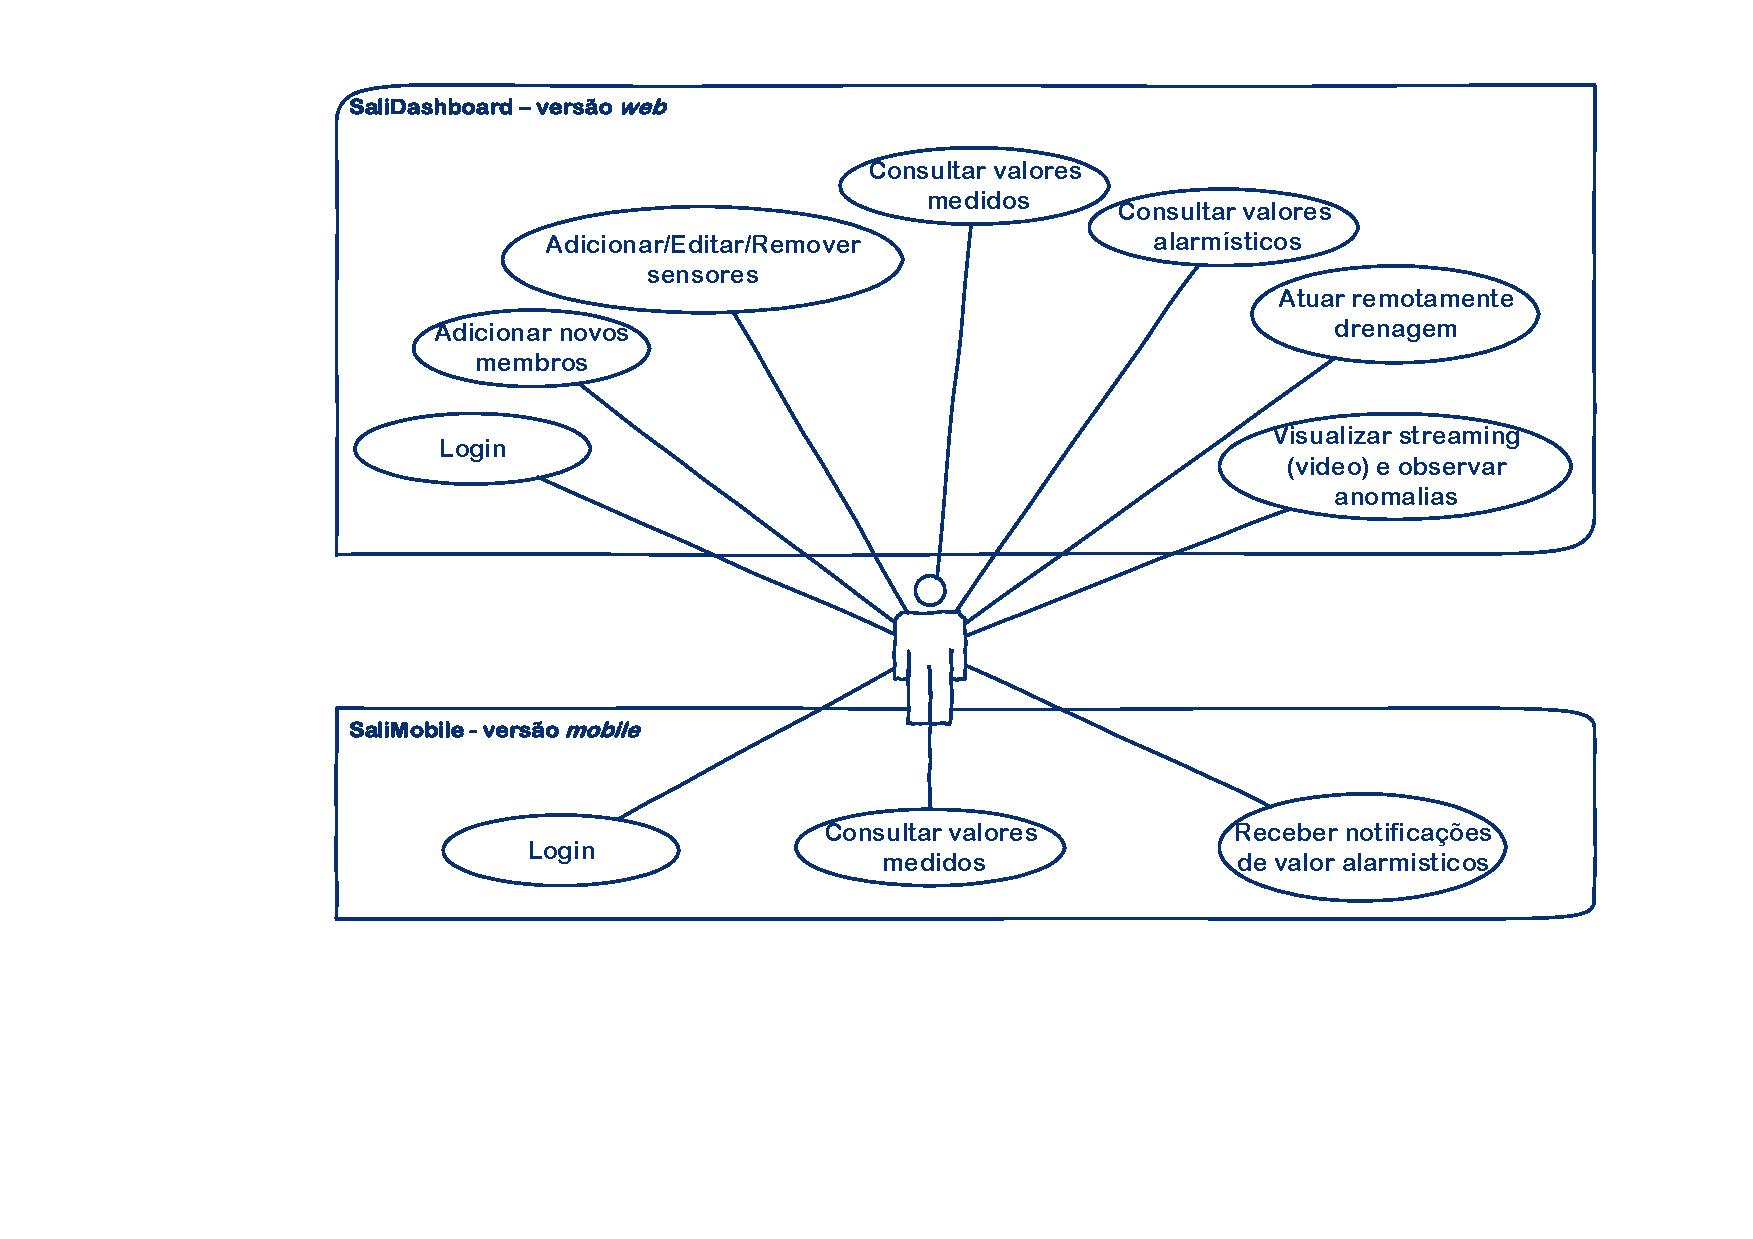
\includegraphics[scale=0.5]{esquemas/usecases.pdf}
	\caption{Pirâmide do conhecimento: modelo DIKW}
	\label{dikw}
\end{figure}











\begin{table}[h]
	\centering
	
	\begin{tabular}{|
			>{\columncolor[HTML]{EFEFEF}}l |l|}
		\hline
		\textbf{Caso de utilização:} & \begin{tabular}[c]{@{}l@{}}-dasdasdasasdasdddddddddddddddddddddddd\\ -dasdasd\\ -dasdasda\end{tabular} \\ \hline
		\textbf{Ator:} &  \\ \hline
		\textbf{Descrição:} &  \\ \hline
		\textbf{Pré-condições:} &  \\ \hline
		\textbf{Pós-condições:} &  \\ \hline
	\end{tabular}
	\caption{Casos de utilização: Login/Logout}
	\label{my-label}
\end{table}




\newpage
\section{Estrutura da base de dados}


\begin{figure}[!htb]
	\centering
	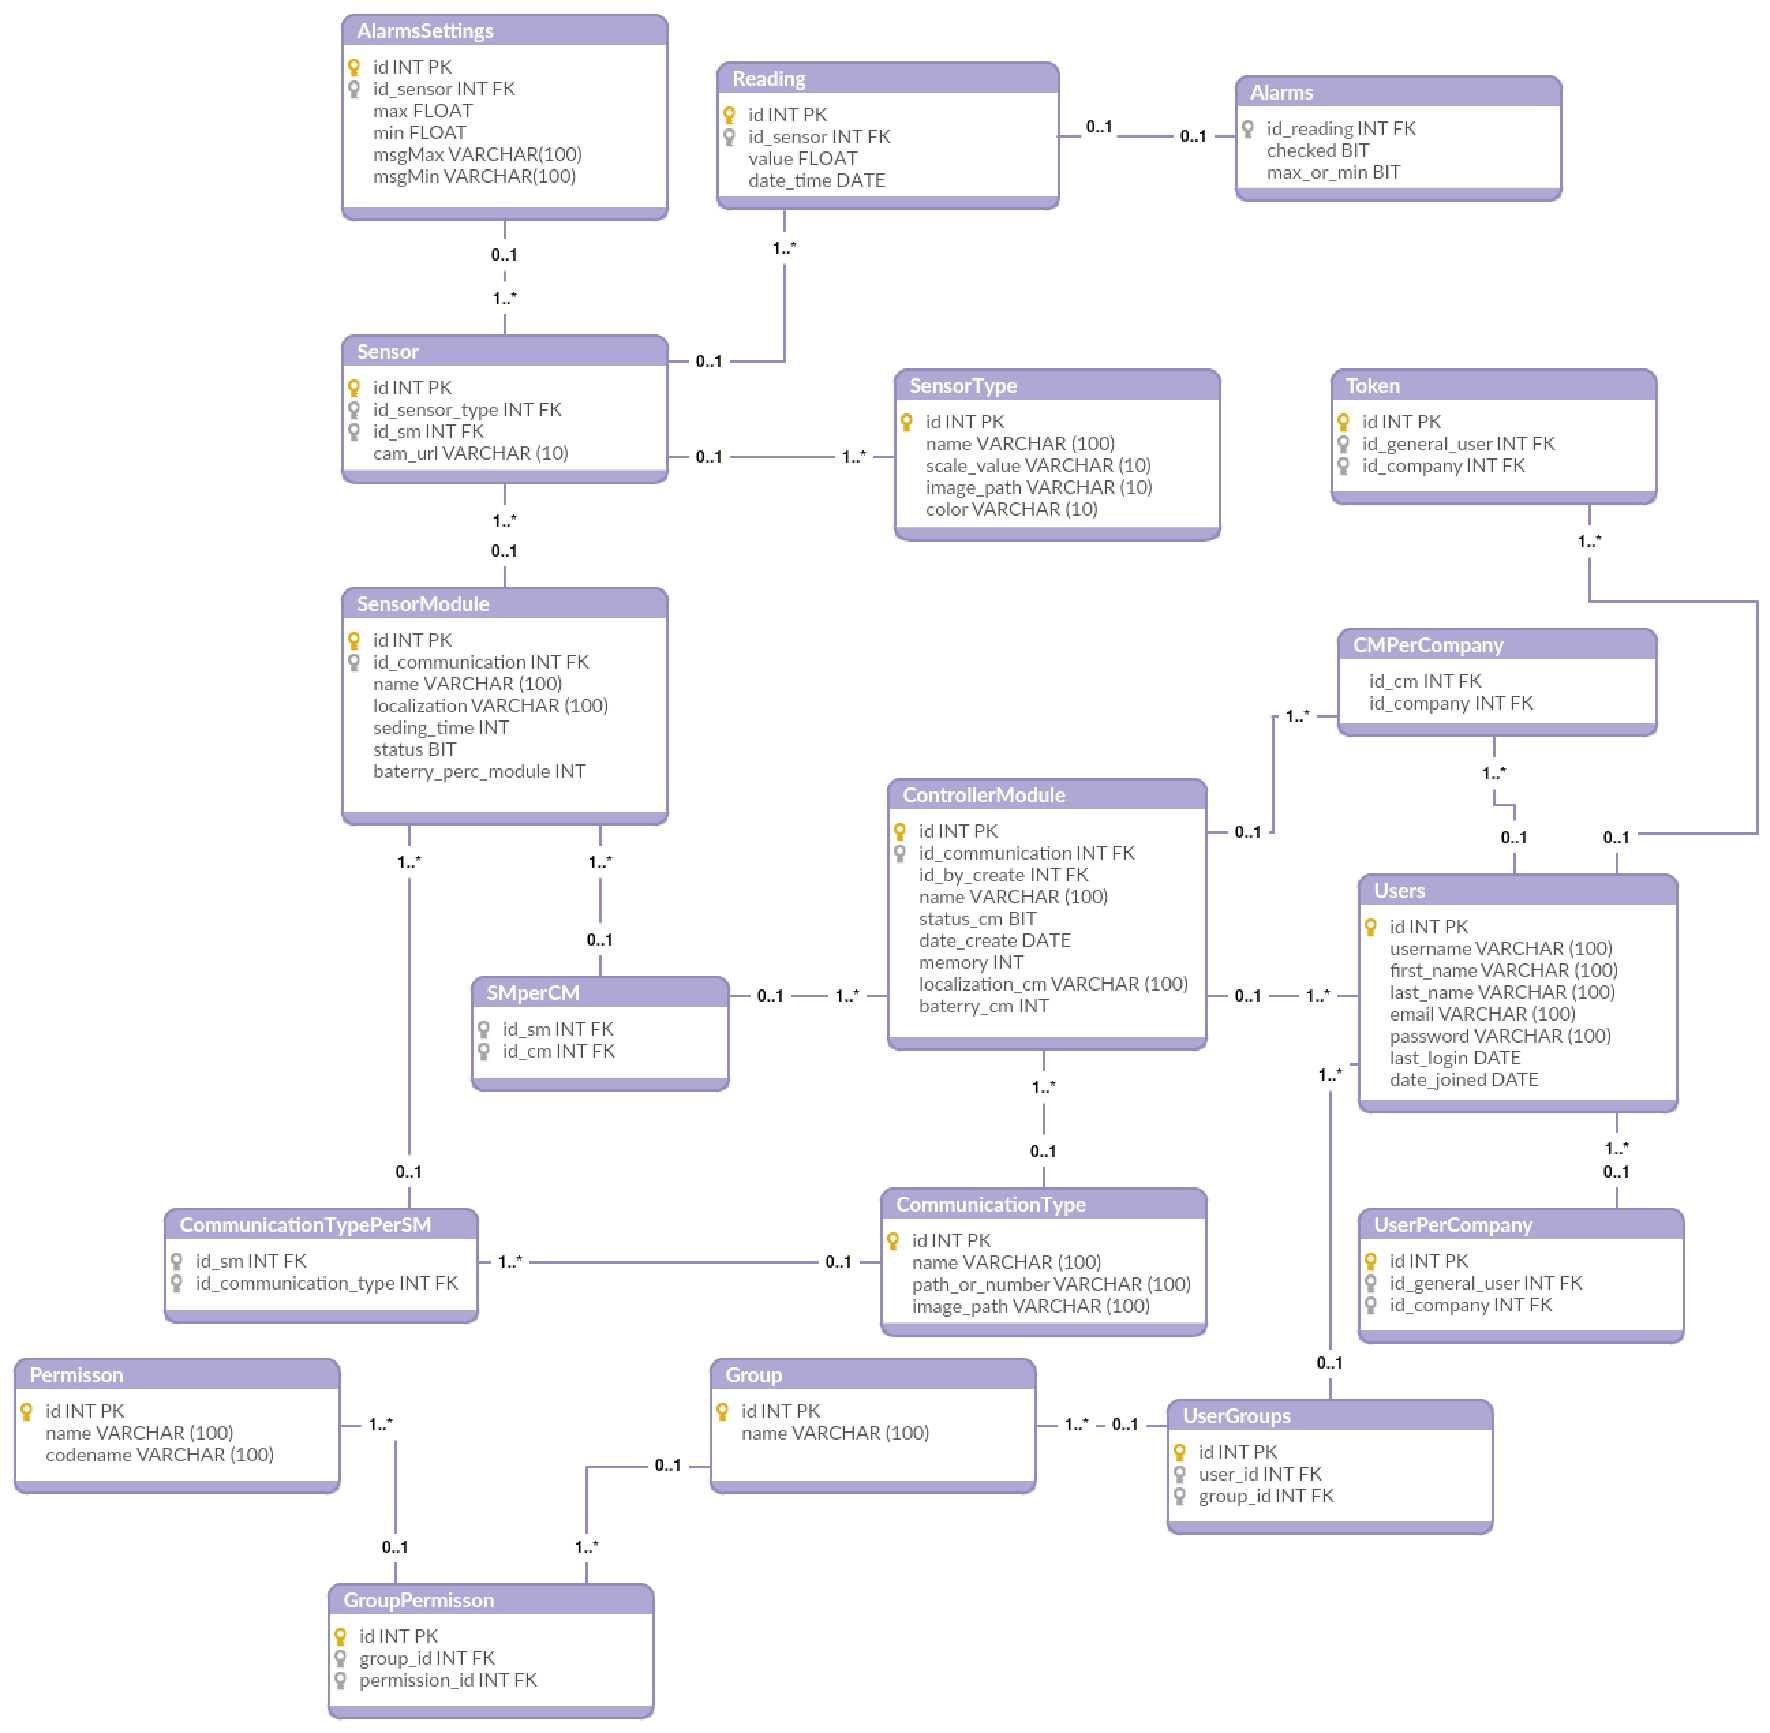
\includegraphics[scale=0.25]{esquemas/database_tese.pdf}
	\caption{Pirâmide do conhecimento: modelo DIKW}
	\label{db}
\end{figure}




\begin{table}[h]
	\centering
	\begin{tabular}{|l|l|l|}
		\hline
		\multicolumn{1}{|c|}{\textbf{Nome}} & \multicolumn{1}{c|}{\textbf{Identificador}} & \multicolumn{1}{c|}{\textbf{Descrição}} \\ \hline
		User & auto-incrementado & dasdas \\ \hline
		ControllerModule&  &  \\ \hline
		SensorModule&  &  \\ \hline
		CommunicationType&  &  \\ \hline
		SensorType&  &  \\ \hline
		Sensor&  &  \\ \hline
		Reading&  &  \\ \hline
		AlarmsSettings&  &  \\ \hline
		Alarms&  &  \\ \hline
	\end{tabular}
	\caption{My caption}
	\label{my-label}
\end{table}






\newpage

\section{Requisitos de funcionamento}


\newpage


\section{API}

Os métodos da API permitem executar as funções REST. Assim, torna-se fundamental perceber estes métodos para ter um melhor conhecimento do funcionamento do sistema. Como tal, de seguida, são descritos os métodos mais importantes que dão suporte a cada uma das funções REST.

\begin{itemize}
	\item \textbf{GET}: 
	\item \textbf{POST}: 
	\item \textbf{DELETE}: 
\end{itemize}





\section{Valores simulados}



\section{\textit{Deploy} do projecto}


https://jee-appy.blogspot.com.tr/2015/04/deploy-django-project-on-apache-using.html

Caracteristicas da maquina virtual

Description:	Ubuntu 14.04.1 LTS
64 bitsRAM 2GB 

\section{Considerações finais}








